\documentclass{beamer}
\begin{document}
\title{Optimizing the software stack of a cosmic proportions cluster of multi-core machines}
\author{Sebastian Pop}
\institute{SARC: Samsung Austin R\&D Center}
\date{February 5, 2017}

\frame{\titlepage}

\frame{\frametitle{Why Optimizing the Android Software Stack?}
  \begin{itemize}
  \item 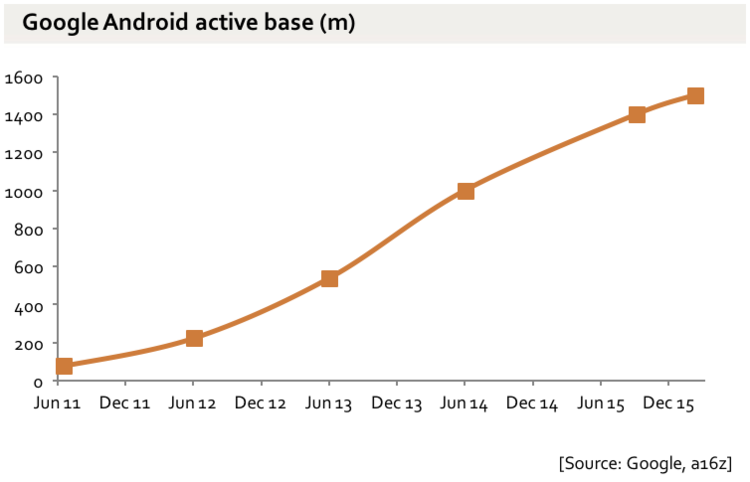
\includegraphics[width=8cm]{active-devices.png}
  \item 1 Watt/device 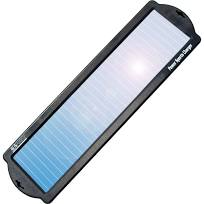
\includegraphics[width=1cm]{1watt.jpg} $\longrightarrow$ 1GW / billion devices 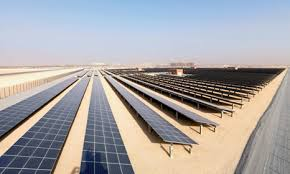
\includegraphics[width=2cm]{1GWatt.jpg}
  \item \$0.10/kWh = \$200M for 1 billion devices / year
  \end{itemize}
}

\frame{\frametitle{Android Open Source Project (AOSP) Software Stack}
  \begin{itemize}
  \item AOSP: common base for Android devices (+ customizations)
  \item C/C++ for the platform libraries, Java for user interface
  \item $\sim80\%$ execution cycles in C/C++, $\sim20\%$ in Java
  \item release/updates/deprecation ($5\sim6$ years) \\
    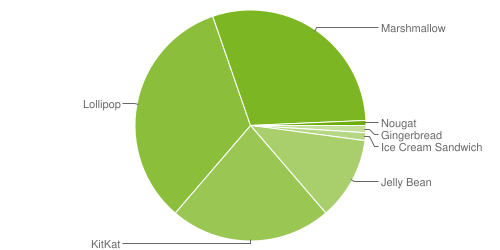
\includegraphics[width=8cm]{android-versions.png} \footnote{Data collected during a 7-day period ending on January 9, 2017.}
  \end{itemize}
}

\frame{\frametitle{Plan}
  \begin{itemize}
  \item Performance analysis
  \item Enable more secure execution environment (CFI)
  \item Enable profile optimizations (AutoFDO)
  \item Improve performance of AOSP libraries
  \end{itemize}
}

\frame{\frametitle{Performance Analysis}
  \begin{itemize}
  \item linux perf: profile of cycles (per function, hot-spots)
  \item valgrind: number of executed instructions (branches, R/W)
  \item static profiles: how many times a function is called
  \end{itemize}
}

\frame{\frametitle{Towards more secure devices}
  \begin{itemize}
  \item Control Flow Integrity (CFI): $2\%$ overhead (\$4M) \footnote{Enforcing Forward-Edge Control-Flow Integrity in GCC\&LLVM, USENIX'14}
  \item to enable on Android: need to further reduce its cost
  \item 
  \end{itemize}
}

\frame{\frametitle{AutoFDO: Feedback Directed Optimization}
  \begin{itemize}
  \item linux-perf extracts profiles of running systems
  \item little to no overhead \footnote{Google Wide Profiling: A Continuous Profiling Infrastructure for Data Centers, IEEE Micro (2010)}
  \item compute basic block frequencies from profiles
  \item better inlining \footnote{Lightweight Feedback-Directed Cross-Module Optimization, CGO 2010}
  \item hot/cold code placement, register allocation, jump-threading
  \end{itemize}
}

\frame{\frametitle{Intel-LBR: Last Branch Record}
  \begin{itemize}
  \item Intel-LBR: records last 16 taken branches
  \item provides precise basic block execution frequency
  \item how do we do this on ARM?
  \end{itemize}
}

\frame{\frametitle{ARM-ETM: Embedded Trace Macrocell}
  \begin{itemize}
  \item ARM-ETM: records execution traces (for debug)
  \item dedicated circular buffer 1 to 3MB ($\sim10^5$ branches/MB)
  \item no overhead
  \item support in Linux kernel by Mathieu Poirier (Linaro)
  \item perf-inject translates execution traces to LBR events
  \item next android kernel linux-4.9 has support for ETM
  \end{itemize}
}

\frame{\frametitle{From Profiles to Power Usage}
  \begin{itemize}
  \item  \footnote{An Analysis of Power Consumption in a Smartphone, USENIX'10}
  \end{itemize}
}

\frame{\frametitle{Improve performance of libraries}
  \begin{itemize}
  \item comparative performance: std-benchmark\footnote{https://github.com/hiraditya/std-benchmark}
  \item std-benchmark provides micro-benchmarks for each function in C/C++ standard libraries
  \item detect room for improvement
    \begin{itemize}
    \item compile with different compilers
    \item link with different standard libraries
    \item run on different machines: CPUs, architectures
    \end{itemize}
  \end{itemize}
}



\end{document}
